\documentclass{article}
\usepackage[utf8]{inputenc}

\usepackage{fancyhdr} 
\usepackage{lastpage} 
\usepackage{extramarks} 
\usepackage{graphicx,color}
\usepackage{anysize}
\usepackage{amsmath}
\usepackage{natbib}
\usepackage{caption}
\usepackage{hyperref}
\usepackage{listings}
\usepackage{float}
\usepackage{url}
\usepackage{listings}

\textwidth=6.5in
\linespread{1.0} % Line spacing
\renewcommand{\familydefault}{\sfdefault}

\newcommand{\includecode}[4]{\lstinputlisting[float,floatplacement=H, caption={[#1]#2}, captionpos=b, frame=single, label={#3}]{#4}}

%% includescalefigure:
%% \includescalefigure{label}{short caption}{long caption}{scale}{filename}
%% - includes a figure with a given label, a short caption for the table of contents and a longer caption that describes the figure in some detail and a scale factor 'scale'
\newcommand{\includescalefigure}[5]{
\begin{figure}[H]
\centering
\includegraphics[width=#4\linewidth]{#5}
\captionsetup{width=.8\linewidth} 
\caption[#2]{#3}
\label{#1}
\end{figure}
}

%% includefigure:
%% \includefigure{label}{short caption}{long caption}{filename}
%% - includes a figure with a given label, a short caption for the table of contents and a longer caption that describes the figure in some detail
\newcommand{\includefigure}[4]{
\begin{figure}[H]
\centering
\includegraphics{#4}
\captionsetup{width=.8\linewidth} 
\caption[#2]{#3}
\label{#1}
\end{figure}
}

%% Code formatting:
\usepackage{xcolor}
\definecolor{light-gray}{gray}{0.95}
\newcommand{\code}[1]{\colorbox{light-gray}{\texttt{#1}}}

%%------------------------------------------------
%% Parameters
%%------------------------------------------------
% Set up the header and footer
\pagestyle{fancy}
\lhead{\authorName} % Top left header
\chead{\moduleCode\ - \assignmentTitle} % Top center header
\rhead{\firstxmark} % Top right header
\lfoot{\lastxmark} % Bottom left footer
\cfoot{} % Bottom center footer
\rfoot{Page\ \thepage\ of\ \pageref{LastPage}} % Bottom right footer
\renewcommand\headrulewidth{0.4pt} % Size of the header rule
\renewcommand\footrulewidth{0.4pt} % Size of the footer rule

\setlength\parindent{0pt} % Removes all indentation from paragraphs
\newcommand{\assignmentTitle}{Assignment 1}
\newcommand{\moduleCode}{CSU33031} 
\newcommand{\moduleName}{Computer Networks} 
\newcommand{\authorName}{Liam Junkermann} 
\newcommand{\authorID}{19300141} 
\newcommand{\reportDate}{\today}

\title{
    \vspace{-1in}
    \begin{figure}[!ht]
    \flushleft
    
\includegraphics[width=0.4\linewidth]{reduced-trinity.png}
    \end{figure}
    \vspace{-0.5cm}
    \hrulefill \\
    \vspace{1cm}
    \textmd{\textbf{\moduleCode\ \moduleName}}\\
    \textmd{\textbf{\assignmentTitle}}\\
    \textmd{\authorName\ - \authorID}\\
    \textmd{\reportDate}\\
    \vspace{0.5cm}
    \hrulefill \\
}
\date{}
\author{}

\begin{document}
    \lstset{language=bash, float=h, captionpos=b, frame=single, numbers=left, numberblanklines=false, numberstyle=\tiny, numbersep=1mm, framexleftmargin=3mm, xleftmargin=5mm, aboveskip=3mm, breaklines=true}
    \captionsetup{width=.8\linewidth} 
    
    \maketitle
    \tableofcontents
    \newpage
    
    \section{Introduction}
    \label{sec:Intro}
    The problem described involved creating a Publish-Subscribe system. In order to complete this, the necessary components needed to be built: the broker, the subscribers, and publishers. The publishers send data to the broker, which then processes and routes the traffic to the appropriate subscribers. The subscribers are allowed to subscribe to a variety of topics, transactions which are also handled by the broker. Through this assignment, the context of a system with various sensors and a dashboard as shown below (from assignment declaration).
    \vspace{0.5cm}
    \begin{center}
        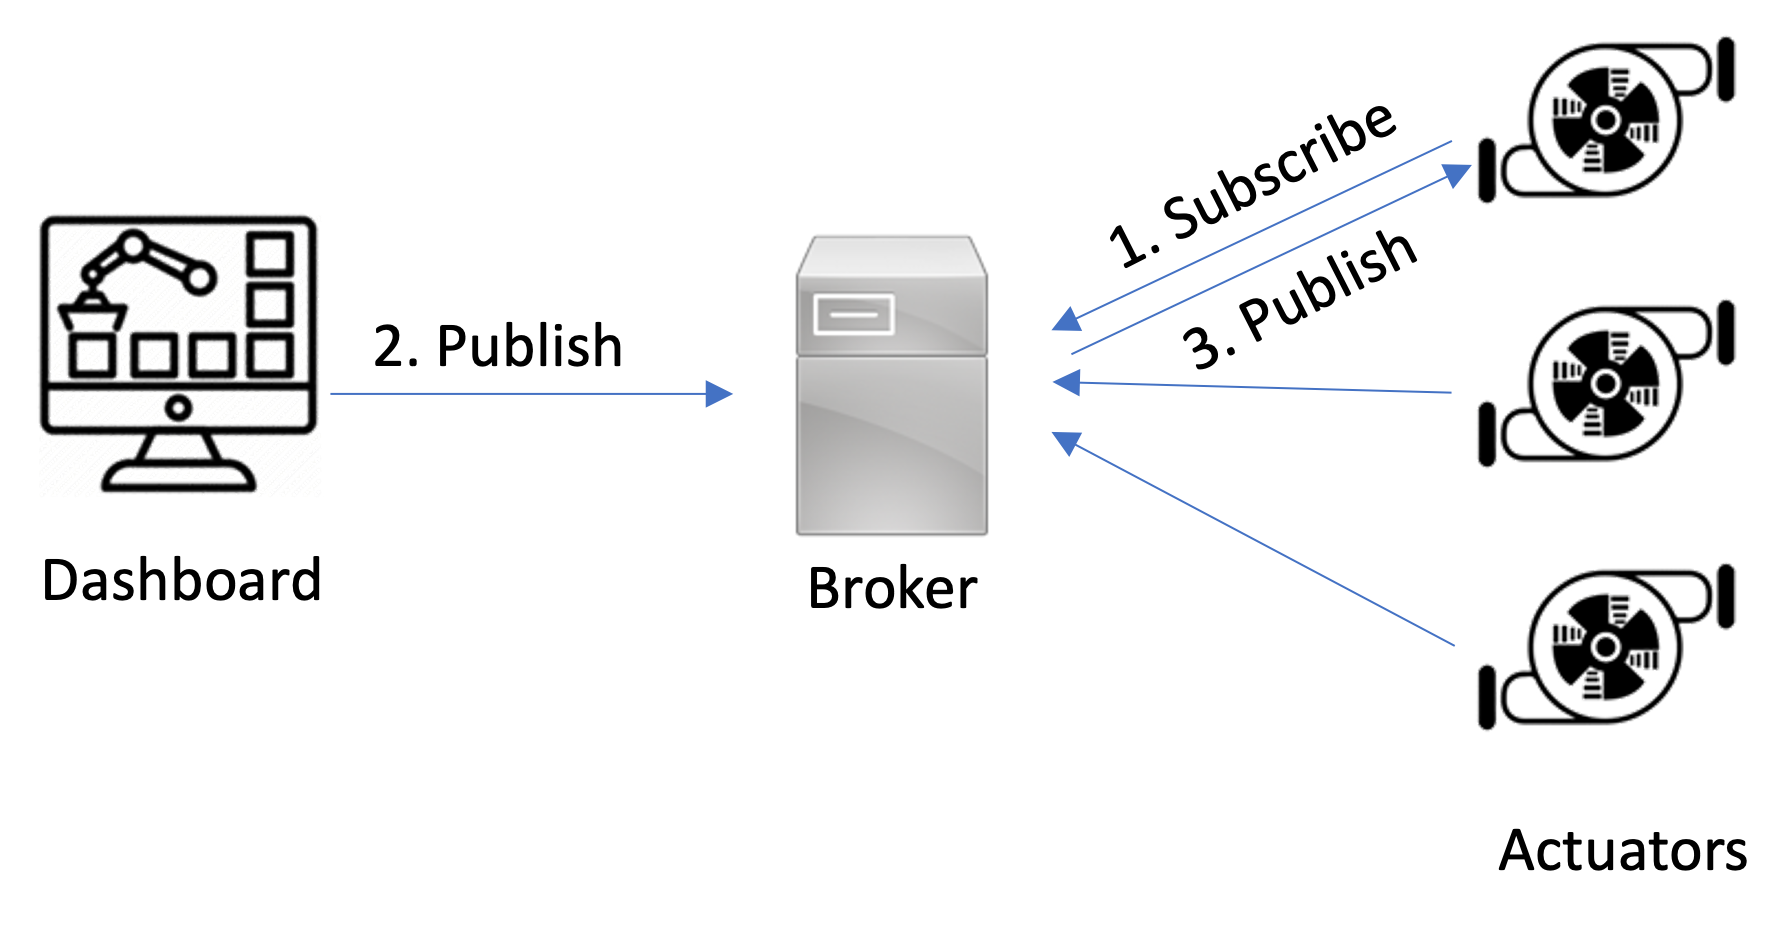
\includegraphics[]{Publish-Instruction-to-Actuators.png}
    \end{center}
    
    \section{Design and Implementation}
    \label{sec:Design}
    A very basic design approach was used. Given that the scope of this project was fairly limited (the context of a few sensors and dashboards) the setup of a prospective system was straight forward with the three clients as described above being built: The broker, the publishers -- in this case the Command and Control (C\&C) module, and the subscribers -- in this case the Client.
    
    \subsection{The Packet structure}
    \label{subsec:PacketStructure}
    Each packet sent is of the same structure and length. The packets each have a header length of 2 bytes which can be assigned to different values depending on the context. There are two types of packet: acknowledgement and data packets. The Data packets are typed by their sender, so any packets from the Broker, Client, or C\&C carry their own value in the first header position. Data packets include data length in the second header byte, while acknowledgement packets have their acknowledgement or acceptance state stored in the second byte of the header.
    
    \subsection{The Communication Method}
    \label{subsec:communication}
    This entire system is written in Java and relies on the \code{java.net.*} packages. All data is transferred through \code{DatagramPackets} with connections to the sockets opened by the nodes. In order to complete packet transactions the source node connects to the target nodes open socket. These socket addresses are hard-coded for the Broker and C\&C modules, the Client nodes are assigned sockets randomly due to the current topology (see \nameref{sec:Topology}).
    
    \subsection{The Broker}
    \label{subsec:Broker}
    The broker is the most complicated part of this service, as its purpose is to handle the traffic from all publishers and subscribers, as well as maintain the packet format. At its core the Broker is just another node, with a Listener for packets, which are then parsed and responded to accordingly. The Broker receives packets from the clients (publishers and subscribers), then respond with an acknowledgement, and if the packet was received from a publisher, the relevant subscribers will then be notified. The Broker sends two types of packets:
    \begin{description}
        \item[Packet Receipt Acknowledgement packet] The first packet the Broker sends is an acknowledgement type packet, declared in the first byte of the header. This packet is sent in response to a packet from either the C\&C Module or the Client module to let them know that the packet has been received. In the case of a packet from the C\&C module being made, this triggers the relevant data packets being sent to the subscriber list as well.
        \item[Broker Data Packet] The other packet the broker sends is a Broker Data Packet, this is defined in the header, with the data length being described in the second header byte. Finally the string value of the C\&C command is added to the data body of the packet, to be sent to the subscribed clients.
    \end{description}
    
    \subsection{Command and Control}
    \label{subsec:C&C}
    The Command and Control (C\&C) module utilises the interactive \code{Terminal} prompt in order to allow the user to issue commands to the necessary clients list. The C\&C module issues one type of packet: 
    \begin{description}
        \item[Command and Control packet] The C\&C packet is sent to the broker with the data headers set to the control value for a C\&C packet and the data length, in each of the header bytes respectively. The packet data is the command which will be relayed to the various listening subscribers.
    \end{description}
    
    \subsection{The Client}
    \label{subsec:Client}
    The Client's sole purpose is to subscribe to the brokers subscription streams, and in a real world application, would use the subscription data to trigger events either with an actuator of some kind. The Client still sends two types of packets:
    \begin{description}
        \item[Connection Packet] The client -- when launched -- immediately begins to try to make a connection with the broker in order to subscribe to a stream. The connection packet attempts to send a packet to the broker to register for the subscription list on the broker side, this then expects an acknowledgment packet response which is confirmed to the actuator through the \code{Terminal}.
        \item[Command response packet] When the client receives a command from the Broker it must acknowledge whether it can accept the job or not. This packet is typed as a \code{Client} packet, with the response data length flag set in the second header position.
    \end{description}
    
    \newpage
    \section{Deployment Topology}
    \label{sec:Topology}
    A very basic deployment approach was used for the duration of this project. Each of the components described above (\nameref{subsec:Broker}, \nameref{subsec:C&C}, and \nameref{subsec:Client}) were deployed in their own docker containers all on their own Docker managed virtual subnet. There was a fourth container which hosted Wireshark to allow the capture of \code{.PCAP} files, due to some of the limitations of virtual networks within MacOS. Each of the containers was named accordingly to allow the hostnames to be hard-coded into the necessary class files (\nameref{subsec:Broker} as \code{broker}, \nameref{subsec:C&C} as \code{CAndC}, and \nameref{subsec:Client} as \code{client}). Currently, there are multiple clients running on the same \code{client} container. \nameref{subsec:Client} class generates 3 clients for testing purposes which all utilise the same container resources.
    
    \begin{center}
        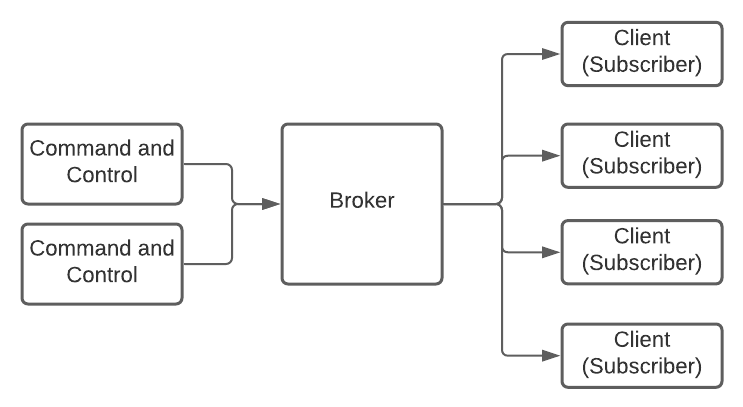
\includegraphics[width=0.7\linewidth]{topography.png}
    \end{center}
    
    \newpage
    \section{Summary and Reflection}
    \label{sec:summary}
    Building this Publish-Subscribe (pubsub) system has been a great learning experience and has allowed me to utilise skills and technologies I have had experience with outside of college to properly work together and produce an interesting final product. Next I will discuss the strengths and weaknesses of the outcome, as well as reflect on my learnings.
    \subsection{The systems strengths and weaknesses}
    The current implementation of the pubsub is very limited. While there was a lot of learning as a result of building this and it works as intended, there are many more features that could have been added to improve or extend the current implementation. Pubsub systems are used regularly in IoT systems with lots of sensors and actuators which work together to control or enhance environments, for example in smart homes. In general, pubsub systems are great when reliability is not crucial to the rest of the system, socket based applications tend to have some packet loss and latency and a broker might not even know it is missing packets from publishers as there is no other mode of communication between the publishers, brokers, and subscribers. That being said, pubsub systems -- like this one and more developed implementations like \href{https://mqtt.org/}{MQTT} -- generally have lower overheads than a \code{TCP} based method with more handshakes and assurances that connections have been made, this makes them quicker in transferring data as well, something that is important when generally small data packets are sent to populate a sensor output, for example. 
    \subsection{Learnings from Assignment 1}
    Having done some work with \hyperlink{https://www.docker.com/}{Docker} and Docker clusters in the past I had a basic knowledge of how networking socket applications worked, this made it easier for me to understand how to work with the pubsub socket system. There were two main struggles when completing this project: 
    \begin{description}
        \item[MacOS and Docker Networks] Because of the way recent releases of MacOS and it's security has been built each application has it's own security container which has limited access to the rest of the machine, this includes Docker. In practice this means that any networks that Docker creates are actually just virtual networks within a virtual machine container managed by MacOS. This meant that Wireshark running on the host machine did not have access to the virtual network created to host the collection of Docker containers which deployed the pubsub system. Unfortunately, it took me far too long to figure out that this was the issue, but once I isolated this problem I was able to fashion a solution using X11 and Wireshark running from a container within the Docker network, allowing me to create the necessary \code{.PCAP} files. 
        \item[Broker not receiving packets] For the longest time, I was having an issue with packets being sent (and picked up by wireshark), but not making it to the Broker -- and as a result not coming back to the C\&C module that sent the first packet. After much debugging I found that I did not correctly implement the \code{Node} module provided, and had missed two lines:
            \begin{lstlisting}[language=java]
                listener.setDaemon(true);
                listener.start();
            \end{lstlisting}
            These two lines were vital to actually listening for packets and once this issue was resolved my implementation worked great.
    \end{description}
    This assignment was very interesting and allowed me to put into context -- and have a much better understanding of -- some other projects and tools I've used for personal projects.
    
\end{document}